\documentclass[12pt]{article}
\usepackage[utf8]{inputenc}
\usepackage{mathptmx} % Times New Roman
\usepackage{amsmath, amssymb, amsthm}
\usepackage{setspace}
\doublespacing
\usepackage{xr}
\externaldocument{supplement_round3}
\usepackage{booktabs}
\usepackage{multirow}
\usepackage{array}
\usepackage{graphicx}
\usepackage{ragged2e}
\usepackage{hyperref}
\hypersetup{hidelinks}
\usepackage[numbers,super]{natbib} % AMA superscript
\usepackage[margin=1in]{geometry}
\usepackage{tikz}

\usetikzlibrary{positioning,arrows.meta}
\newcommand{\keywords}[1]{\vspace{0.5em}\noindent\textbf{Keywords:} #1}

\title{\textbf{Anchoring Large Language Models to Empirical Behavioral Evidence}\\[0.5em]
\large A Hybrid Approach for DCE-Grounded Narrative Policy Simulation}
\author{Blinded for peer review}
\date{}

\begin{document}

\maketitle


\begin{abstract}\justifying
\textbf{Objective:} To develop and validate EFR (EFR), an inference-time procedure anchoring LLM outputs to a DCE-estimated reference surface without retraining.

\textbf{Methods:} A Wuhan vaccination DCE ($N\!=\!1{,}027$) was combined with LLM simulation on a 64-state policy grid. EFR computes $\pi_{\text{EFR}} = \lambda\,\bar\pi_{\text{LLM}} + (1-\lambda)\,P_{\text{emp}}$ with $\lambda\!=\!0.25$ fixed as a conservative operating point.

\textbf{Results:} Held-out validation on six DCE choice tasks ($N=205$ respondents) shows multinomial log loss: Pure-DCE $0.911$, EFR $0.923$, Raw LLM $1.020$. EFR reduced log loss by $9.5\%$ versus Raw LLM and approached Pure-DCE performance (within $1.3\%$). The unconstrained LLM violated waiting-time monotonicity on $62.5\%$ (Qwen2.5-72B), $34.4\%$ (DeepSeek V4 Pro), and $10.4\%$ (MiroThinker) of scenarios; after EFR, MVR-Wait dropped to $30.2\%$, $7.3\%$, and $8.3\%$ respectively. Rank correlation $\rho$ rose from $0.061$/$0.302$/$0.531$ (Raw) to $0.689$/$0.812$/$0.756$ (EFR), all exceeding the uniform-noise null ($\rho\!=\!0.366$, $95\%$ CI $[0.148, 0.560]$); two of three models also exceeded the stricter permutation null that preserves the LLM's marginal distribution (Supplement B).

\textbf{Limitations:} Single-site DCE; respondent-level holdout evaluates generalization to unseen respondents, not unseen tasks. Out-of-design scenarios lacked human ground truth.

\textbf{Conclusion:} EFR constrains LLM outputs to a DCE-derived frontier, bounding deviation while preserving narrative-extension capability. It is a wrapper for DCEs, not a replacement.
\end{abstract}


\keywords{EFR; large language models; discrete choice experiment; health technology assessment; behavioral simulation}

\clearpage

\section*{Highlights}
\begin{enumerate}
    \item EFR is an inference-time regularization layer that constrains LLM outputs to a DCE-estimated reference without retraining.
    \item On held-out respondent validation, EFR recovers most of DCE model\'s predictive performance while retaining a bounded LLM component.
    \item EFR improves structural consistency (monotonicity, rank order) but does not establish behavioral validity for out-of-design narrative scenarios.
\end{enumerate}

\vspace{1em}
\noindent\textbf{Article Type:} Methodological Article

\clearpage
\section{Introduction}
\label{sec:intro}

Large language models (LLMs) are increasingly used as simulated decision-makers for healthcare policy~\citep{Park2023a, Mu2024, VonHoene2025}. Their appeal is that they can interpret rich natural-language scenarios that conventional structured decision models cannot. However, linguistic fluency does not guarantee behavioral reliability: an unconstrained LLM may assign higher acceptance to a longer-waiting policy than to an otherwise identical shorter-waiting policy, contradicting empirically preference patterns and producing unreliable policy rankings.

Current approaches do not explicitly enforce DCE-estimated behavioral constraints~\citep{Aher2022TuringExperiments, Horton2023, santurkar2023whose}: LLM agents may produce decisions that appear linguistically plausible while violating basic preference relationships implied by human behavior.

One source of such constraints is the discrete choice experiment (DCE), which estimates how human preferences vary with decision attributes~\citep{Chan2024}. In this study, we treat DCEs not as models to be replaced by LLMs, but as sources of DCE-estimated behavioral reference. A DCE-estimated choice frontier defines the preference ordering and directional relationships supported by responses. The challenge is to combine this empirical behavioral knowledge with the representational flexibility of LLMs, so that simulated predictions can incorporate an LLM-derived narrative component while remaining closer to DCE-implied structure; whether the resulting narrative extension is behaviorally more accurate on out-of-design scenarios is not established by the present study, because no human ground truth is available outside the original DCE design space.

We propose a \textbf{hybrid approach} that anchors LLM-generated choice probabilities to empirical behavioral evidence from DCEs. The method estimates an empirical choice frontier from DCE responses and blends the LLM's raw probability with the frontier through a transparent weighted-averaging procedure. The adjustment is auditable: the raw LLM probability, the empirical frontier value, the blending weight, and the final adjusted probability are all directly inspectable. The method requires no retraining. The same LLM can be anchored using different empirical datasets, enabling domain-specific grounding while preserving general capabilities.

We evaluate the approach using a real-world vaccination-timing DCE involving 1,027 adults in Wuhan, China. This study makes three contributions:

\begin{enumerate}
    \item We introduce a lightweight inference-time adjustment procedure for grounding LLM-based simulation in empirically estimated human behavioral knowledge.

    \item We show that the proposed adjustment improves structural consistency across multiple LLMs, reducing behavioral inconsistencies and improving agreement with the DCE-estimated reference. On held-out-respondent validation (local Ollama Qwen2.5-72B replication), EFR materially improved predictive performance relative to the unconstrained LLM ($9.5\%$ reduction in log loss) and approached the Pure-DCE model (within $1.3\%$), while retaining a non-zero LLM component. \textbf{The retention of an LLM component is motivated by narrative-extension capability, not by evidence that LLMs provide accurate behavioral simulation for novel scenarios; the OOD evaluation demonstrates constraint effects, not validation of LLM behavioral accuracy.}

    \item We demonstrate that empirically grounded behavioral models can be extended to richer natural-language healthcare policy scenarios while preserving auditable behavioral constraints.
\end{enumerate}\section{Related Work}

Our work connects two research areas: LLM-based synthetic agents for healthcare simulation and empirical behavioral models derived from discrete choice experiments (DCEs). While these two directions have developed largely independently, both seek to improve the realism and reliability of decision support. Our work lies at their intersection by incorporating empirically estimated behavioral knowledge into LLM-based synthetic agents through inference-time regularization.

\emph{Prior LLM-for-HTA work in this journal.} Recent issues of \emph{Value in Health} have featured LLMs along trajectories distinct from the behavioral-simulation axis we pursue: evidence extraction~\citep{shree2025stability}, sponsor--HTA conversation simulation~\citep{luo2025sponsor}, microsimulation~\citep{tornberg2025validation}, and LLM-based prediction of stated preferences~\citep{Cheng2026}. We deploy LLMs as narrative-extension mechanisms anchored to a DCE-derived empirical frontier, not as tools for review or negotiation. The closest analogue outside HTA is Twin-2K-500~\citep{toubia2025twin}, which validates LLM-as-consumer simulation in marketing; we extend this line to health policy. A pre-existing LLM-powered social digital twin framework~\citep{koaik2026social} is conceptually adjacent but does not anchor to a pre-collected empirical choice frontier.

\subsection{LLM-Based Synthetic Agents}

Large language models (LLMs) have enabled a new generation of synthetic agents capable of generating natural-language reasoning and simulating human decision making across diverse domains~\citep{Bommasani2021, Park2023a, Mu2024}. In healthcare, these agents have been explored for public health communication, policy evaluation, and behavioral simulation~\citep{Sehgal2025, Gullison2025}. Their principal advantage is representational flexibility: unlike conventional statistical models, LLMs can process rich textual descriptions and respond to scenarios that extend beyond predefined structured variables.

However, behavioral realism remains a major challenge: LLM responses may violate expected directional relationships (e.g., waiting-time monotonicity, where longer waits should reduce acceptance) or produce implausible preference orderings~\citep{Aher2022TuringExperiments, Horton2023, hintze2025nonlinear}. Prompt engineering can reduce some inconsistencies but provides no explicit mechanism for enforcing behaviorally grounded constraints~\citep{wang2025simulate, wang2025heating}; the mechanism cannot guarantee compliance across diverse narrative phrasings outside the original prompt template. We adopt the LLM-as-narrative-component framing of~\citet{Argyle2023, Horton2023}: the LLM's narrative output is one input to a convex blend with an empirical choice frontier, not a stand-alone behavioral model.

\subsection{Empirical Behavioral Models from Discrete Choice Experiments}

Discrete choice experiments (DCEs) provide a well-established framework for estimating how individuals trade off policy-relevant attributes such as waiting time, vaccine efficacy, side effects, and financial incentives~\citep{Soekhai2019a, Chan2024}. Under the random utility framework~\citep{Train2009, louviere2000stated}, DCE responses can be used to estimate an empirical choice frontier that preserves interpretable relationships between decision attributes and choices. Mixed-logit models further account for preference heterogeneity across respondents~\citep{hensher2003mixed, hensher2015applied}.

In this study, we treat the DCE frontier as an empirically estimated source of behavioral knowledge rather than as assumption-free ground truth. While empirical choice models provide transparent and behaviorally interpretable predictions within their original experimental design, they cannot directly operate on rich natural-language policy scenarios.

\subsection{Bridging Empirical Behavioral Models and LLM-Based Agents}

Existing LLM-based synthetic agents provide representational flexibility but lack mechanisms for enforcing empirically estimated behavioral constraints\citep{li2026position, tornberg2025validation}. DCE-derived behavioral models provide transparent and interpretable structure but remain confined to their experimental design. Existing approaches trade flexibility for reliability or vice versa.

\section{Methods}
\label{sec:methods}

This study integrated two methodological components: (1) a discrete choice experiment to estimate empirical vaccination preferences, and (2) a procedure for aligning LLM predictions with these empirical patterns. The following sections describe each component and the validation approach.

\subsection{Overview}

Section~\ref{sec:stage1} describes the DCE design and empirical frontier; Section~\ref{sec:stage3} presents the EFR framework. Section~4.2 reports the 64-state evaluation, and Section~4.3 reports the out-of-design narrative evaluation; Section~\ref{sec:conclusion} concludes.

\subsection{Stage 1: Empirical Behavioral Knowledge Extraction}
\label{sec:stage1}

The first stage extracts empirical behavioral knowledge from a vaccination-timing DCE conducted among 1,027 adults in Wuhan, China (fielded December 2022--January 2023). This knowledge is an empirical choice frontier that serves as the behavioral reference for inference-time regularization.

\paragraph{DCE design and sampling.}

The Wuhan vaccination-timing DCE used a \textbf{non-orthogonal fractional design} with five policy-relevant attributes: waiting time (0, 1, 3, 6 months), vaccine efficacy (50\%, 70\%, 95\%), side-effect risk (0.1\%, 1\%, 10\%), cash incentive (50, 200, 800 RMB), and vaccine origin (Domestic, Imported). The intended non-opt-out candidate space contained 216 profile cells ($4 \times 3 \times 3 \times 3 \times 2$). All 1,027 respondents each completed \textbf{six randomized choice tasks} drawn from the full factorial design, with each task presenting two non-opt-out alternatives and an opt-out alternative; the design covered 12 of the 216 candidate cells (5.6\% coverage). Task presentation order was randomized across respondents to mitigate order effects. The design was generated using D-efficiency criteria with prior parameter estimates from pilot data; a post-hoc dominance audit confirmed that none of the administered A-versus-B profile pairs exhibited strict dominance across the monotonic attributes.

\paragraph{Sampling and ethics.}

Respondents were recruited through an online panel provider (quota sampling: age 18--65, stratified by gender and education to approximate Wuhan adult population distribution). Eligibility criteria: adult resident of Wuhan, no prior COVID-19 vaccination. The full DCE questionnaire and recruitment protocol are available in the public repository. Individual-level DCE responses are not publicly released because of participant confidentiality. The study was reviewed and approved by the relevant institutional ethics committee, and all participants provided informed consent before participation.

\paragraph{Stakeholder involvement and instrument design.}

Two physician interviews and two rounds of twelve cognitive interviews (ISPOR good-research-practices~\citep{Johnson2013DCE,Bridges2013DCE}) refined the choice-task framing.

\paragraph{Construction of the Empirical Behavioral Reference.}

The behavioral reference was constructed from a 6-parameter grouped/conditional logit with five attribute coefficients and an opt-out alternative-specific constant, estimated on the Wuhan DCE. The frontier maps each candidate policy to a DCE-implied binary policy-versus-opt-out probability (i.e., the probability of choosing the policy alternative over the opt-out under the conditional logit model), providing a deterministic signal that anchors the LLM's narrative choices.

\subsection{Stage 2: Inference-Time Adjustment Procedure} The adjustment algorithm aligns LLM outputs with the empirical reference by computing $\pi_{\mathrm{adj}}(y=1\mid\mathbf{x}_g) = \lambda \cdot \pi_{\mathrm{LLM}}(y=1\mid\mathbf{x}_g) + (1-\lambda) \cdot P_{\mathrm{emp}}(y=1\mid\mathbf{x}_g)$ (the EFR equation $\pi_{\mathrm{adj}} = \lambda \pi_{\mathrm{LLM}} + (1-\lambda) P_{\mathrm{emp}}$; full derivation in Appendix~A.1 of the Supplementary Material). This binary policy-versus-opt-out formulation is the primary definition; for the exact-task categorical validation, EFR is extended to a convex blend of full three-alternative probability vectors (Appendix~N of the Supplementary Material).
\label{sec:stage3}

The final stage applies the adjusted probability to policy evaluation, comparing policy scenarios and estimating changes in expected choice probability.

For a baseline scenario $\mathbf{x}$ and an intervention that changes attribute $x_k$ to $x_k'$, the policy response is:

\[
\Delta_k(\mathbf{x}) = \pi_{\mathrm{adj}}(y=1\mid\mathbf{x}') - \pi_{\mathrm{adj}}(y=1\mid\mathbf{x}),
\]

where $\mathbf{x}'$ denotes the post-intervention scenario. Averaging over comparable scenarios gives the mean policy response for attribute $k$.

Because evaluation operates only on the adjusted probability surface, the approach can be deployed locally without transmitting individual-level DCE responses to external providers. The resulting policy-response quantities are descriptive summaries and should not be interpreted as causal treatment effects.



\clearpage

\clearpage
\section{Experimental Evaluation}

\subsection{Experimental Setup}
\label{sec:setup}

We evaluated EFR using three open-source LLMs (Qwen2.5-72B-Instruct, DeepSeek V4 Pro, MiroThinker-1.7-mini; endpoint and access details in Table~S2). Decoding parameters were matched across models where the API permitted, with Qwen2.5-72B-Instruct and DeepSeek V4 Pro sampled at $\mathrm{temperature}=0.7$, $\mathrm{top\_p}=1.0$, $\mathrm{max\_new\_tokens}=512$, and $R=10$ repeated generations per state to average out sampling noise; MiroThinker-1.7-mini was sampled at $\mathrm{temperature}=0.0$ (deterministic), $\mathrm{top\_p}=1.0$, $\mathrm{max\_new\_tokens}=256$, and $R=10$ repetitions. The empirical choice frontier was estimated from a corrected 6-parameter grouped/conditional logit with five attribute coefficients and an opt-out alternative-specific constant on the full Wuhan DCE sample ($N=1{,}027$ respondents) on vaccination timing (ISPOR good-research-practices~\citep{Johnson2013DCE,Hauber2016DCE}). All LLM evaluations comply with the ViH/ISPOR ELEVATE-GenAI reporting framework (Appendix~C).

\subsection{Behavioral Consistency with the Empirical Frontier}
\label{sec:behavioral_consistency}

\begin{table*}[!htbp]
\centering
\caption{Behavioral consistency with the DCE-estimated reference before and after EFR on the 64-state grid. The reference surface is the DCE-estimated conditional-logit model evaluated on the grid attributes (wait $\in \{0,2,4,6\}$, efficacy $\in \{0.3,0.5,0.7,0.9\}$, side-effect level $\in \{0,1,2,3\}$; cash and origin held at reference values). This is a \textbf{structural diagnostic} on a model-implied projection surface; the grid extends beyond the directly administered DCE profiles. Spearman's $\rho$ measures alignment with the DCE-estimated reference; the exact-task categorical validation (Figure~\ref{fig:heldout_predictive}) is the primary held-out benchmark.}
\label{tab:behavioral_alignment}

\begin{tabular}{llcccc}
\toprule
Model & Method & MSE $\downarrow$ & MAE $\downarrow$ & MVR-Wait (\%) $\downarrow$ & Spearman's $\rho$ $\uparrow$\\
\midrule

Qwen2.5-72B-Instruct
& Raw LLM
& 0.0258
& 0.1269
& 62.5
& $+0.061$ \\

& EFR
& 0.0016
& 0.0317
& 30.2
& 0.689 \\

\addlinespace

DeepSeek V4 Pro
& Raw LLM
& 0.0379
& 0.1570
& 34.4
& 0.302 \\

& EFR
& 0.0024
& 0.0392
& 7.3
& 0.812 \\

\addlinespace

MiroThinker-1.7-mini
& Raw LLM
& 0.0872
& 0.2644
& 10.4
& 0.531 \\

& EFR
& 0.0054
& 0.0661
& 8.3
& 0.756 \\

\bottomrule
\end{tabular}
\end{table*}

Table~\ref{tab:behavioral_alignment} summarizes behavioral consistency on the 64-state evaluation grid. The grid attributes extend beyond the directly administered DCE profiles; the reference surface is a DCE-estimated conditional-logit projection. MVR is the wait-axis monotonicity violation rate; $\rho$ is Spearman's rank correlation between $\pi$ and $P_{\text{emp}}$. The exact-task categorical validation (Figure~\ref{fig:heldout_predictive}) is the primary held-out benchmark. EFR ($\lambda = 0.25$) reduced MSE by 94\%, MAE by 75\%, and MVR-Wait substantially; all EFR predictions achieved $\rho \approx 0.69$ or higher, exceeding the uniform-noise null. The permutation null (Supplement B) distinguishes models whose LLM component shows detectable DCE-aligned rank information beyond mechanical anchoring (DeepSeek V4 Pro, MiroThinker; $p \leq .003$) from those that do not (Qwen2.5-72B; $p = .179$; evaluated on the local replication that reproduced the canonical $\rho = 0.689$). Alternative-level analysis: Table~S7.

\clearpage
\subsection{Out-of-Design Policy Scenario Evaluation}
\label{sec:out_of_design}

We evaluated EFR on 20 narrative policy scenarios extending beyond the DCE design (Table~\ref{tab:out_of_design}). Panel A (six pairs) varies waiting time; Panel B (14 pairs) varies other attributes. Full scenario descriptions are provided in the Supplement.

\begin{table}[t]
\centering
\caption{Behavioral consistency under out-of-design policy scenarios.}
\label{tab:out_of_design}
\small
\setlength{\tabcolsep}{4pt}
\begin{tabular}{@{}llccc@{}}
\toprule
Model & Method & MVR ($\downarrow$) & MAD ($\downarrow$) & Spearman $\rho$ ($\uparrow$)\\
\midrule

\multicolumn{5}{l}{\textit{Panel A: Core scenarios (6 paired policy descriptions)}}\\

Qwen2.5-72B-Instruct
& Unconstrained LLM
& 0.333 (2/6)
& 0.290
& 0.12 \\

Qwen2.5-72B-Instruct
& EFR
& 0.000
& 0.072
& 0.87 \\

DeepSeek V4 Pro
& Unconstrained LLM
& 0.667 (4/6)
& 0.257
& $-0.07$ \\

DeepSeek V4 Pro
& EFR
& 0.000
& 0.064
& 0.87 \\

\midrule

\multicolumn{5}{l}{\textit{Panel B: Extended scenarios (14 paired; MVR-Wait defined only for 2 wait-varying pairs)}}\\

Qwen2.5-72B-Instruct
& Unconstrained LLM
& 0.000 (0/2)
& 0.125
& $-0.01$ \\

Qwen2.5-72B-Instruct
& EFR
& 0.000
& 0.031
& 0.93 \\

DeepSeek V4 Pro
& Unconstrained LLM
& 0.000 (0/2)
& 0.209
& $-0.06$ \\

DeepSeek V4 Pro
& EFR
& 0.000
& 0.052
& 0.88 \\

\bottomrule
\end{tabular}

\vspace{0.4em}

\begin{minipage}{0.95\textwidth}
\small
\textit{Note.}
MVR-Wait on wait-varying pairs; MAD/$\rho$ on narrative-only pairs. Panel B $\rho$ reported descriptively (ties affect correlation).
\end{minipage}
\end{table}

In OOD Panel A, raw LLMs violated waiting-time ordering (Qwen: 2/6; DeepSeek: 4/6); EFR eliminated violations and increased rank agreement.

In Panel B, unconstrained LLM rank agreement fell to near zero; EFR maintained zero violations on wait-varying pairs (0/2). Rank agreement was $\rho = 0.93$ (Qwen) and $\rho = 0.88$ (DeepSeek). \textbf{Critical limitation}: These results characterize \emph{structural consistency} with the DCE-estimated reference surface, not \emph{behavioral validity} for human responses to out-of-design narratives. Whether EFR's narrative extension improves behavioral accuracy on novel scenarios---as opposed to merely preserving rank order---awaits human ground-truth validation.




\subsection{Policy Ranking Consistency}
\label{sec:policy_ranking}

EFR increased policy-ranking agreement (PRC: 0.33$\to$0.87, 0.13$\to$0.60, 0.53$\to$0.80). Structural diagnostic, not independent validation.

\section{Discussion}
\subsection{Principal Findings}

EFR improves behavioral consistency without retraining. \emph{First}, raw LLMs showed high monotonicity violations (10--62\%) and weak rank correlation. \emph{Second}, EFR reduced violations to 7--30\% and raised $\rho$ to $\geq 0.69$. Held-out validation: EFR improved log loss versus Raw LLM ($-0.097$; 95\% CI $-0.147$ to $-0.047$). \emph{Third}, policy-ranking agreement increased (Table~S7); this is a structural diagnostic, not independent validation.

\subsection{Methodological Contributions}

Our contribution is \emph{inference-time empirical regularization}: aligning LLM decisions with estimated behavioral structure without model retraining. EFR is a wrapper applicable to any LLM and any choice frontier. The convex combination $\pi_{\mathrm{EFR}} = \lambda \pi_{\mathrm{LLM}} + (1-\lambda) P_{\mathrm{emp}}$ is the simplest anchor; future work could explore non-convex alternatives (Supp. Mat.).

\paragraph*{Attribution and the DCE-dominant mechanism.} The EFR blend ($\lambda = 0.25$) assigns 75\% of the weight to $P_{\mathrm{emp}}$ and only 25\% to LLM component. The improvement in held-out log loss (EFR 0.923 vs.\ Raw LLM 1.020) derives primarily from empirical frontier's signal rather than from LLM narrative understanding. Table~S6 confirms this interpretation: $\lambda = 0.00$ (Pure-DCE) achieves the best predictive performance (0.911), and held-out metrics generally worsen monotonically as $\lambda$ increases. EFR does not outperform the underlying DCE model; its value lies in enabling narrative extension while recovering \emph{most} (not all) of DCE model's predictive performance. The LLM component is permitted only inside the convex blend with $P_{\mathrm{emp}}$; whether it contributes accurate behavioral simulation for novel scenarios---as opposed to merely enabling textual variation---awaits human validation.

A stress test on Panel B (4,800 prompts) showed Qwen2.5-7B constant outputs and DeepSeek V4 0\% parse on N1. \emph{These failures are a safety property, not evidence of LLM value-add}: when LLM output is degenerate, EFR continues to assign 75\% of the weight to $P_{\text{emp}}$, bounding---but not eliminating---LLM component (EFR is not a reliability gate, and the $\lambda=0.25$ weight is fixed rather than adaptive).

\subsection{Implications for Health Policy Analysis}
\label{sec:impl_policy}

EFR offers three HTA implications. \emph{First}, low-cost narrative-policy simulation using DCEs. \emph{Second}, extended DCE applicability to narrative descriptions outside administered profiles. \emph{Third}, suited to early-stage screening; high-stakes decisions require triangulation with traditional methods.

\paragraph*{Limitations and design considerations.} \emph{(i) Wuhan DCE, single-jurisdiction sample.} The reference surface is estimated from one DCE fielded in a single Chinese city (collection period and full DCE questionnaire reported in the public code repository at \url{https://github.com/REDACTED/behavioral-digital-twins}); preference stability across pandemic phases is not established. Replication across additional jurisdictions and time periods is planned future work (Conclusion). \emph{(ii) Conditional-logit specification and frontier stability.} The static frontier uses a 6-parameter grouped/conditional logit (five attribute coefficients plus an opt-out alternative-specific constant) on the full DCE sample, not a random-coefficients mixed logit. Bootstrap ($n=2{,}000$) confirms frontier stability (Supp. Mat. J). The corrected opt-out ASC narrows $P_{\mathrm{emp}}$ to $[0.47, 0.64]$; we trade within-DCE-design contrast for a behaviorally honest specification. \emph{(iii) \(\lambda = 0.25\) as an illustrative conservative operating point.} $\lambda=0.25$ is a fixed conservative operating point (not test-optimized); held-out metrics were not used for selection (Supplementary Material F). \textbf{The paper's substantive conclusions derive from the full $\lambda$ sensitivity analysis (Supplementary Material F.3), not from the specific value $\lambda = 0.25$.} \emph{(iv) Inference-time regularization vs.\ retraining.} EFR is a convex combination of two streams, not a learned gate; non-convex anchors (mixture-of-experts gating, Bayesian shrinkage toward $P_{\mathrm{emp}}$ priors) remain future work.

\subsection{Why Not Use the Discrete Choice Model Alone?}
\label{sec:why_not_dce}

EFR trades exact-task predictive performance for narrative-policy evaluation capability (multinomial log loss: Pure-DCE $0.911$; EFR $0.923$; Raw LLM $1.020$; uniform benchmark $1.099$). \textbf{EFR materially improved exact-task predictive performance relative to the unconstrained LLM} ($9.5\%$ reduction in log loss) and approached the predictive performance of the Pure-DCE model (within $1.3\%$), while retaining a non-zero LLM component for narrative extension. The NDS pilot ($n=2$) illustrates mechanism only (Supp. Mat.). \textbf{Figure~\ref{fig:heldout_predictive}} reports the exact-task categorical held-out validation results.

\begin{figure}[h]
\centering
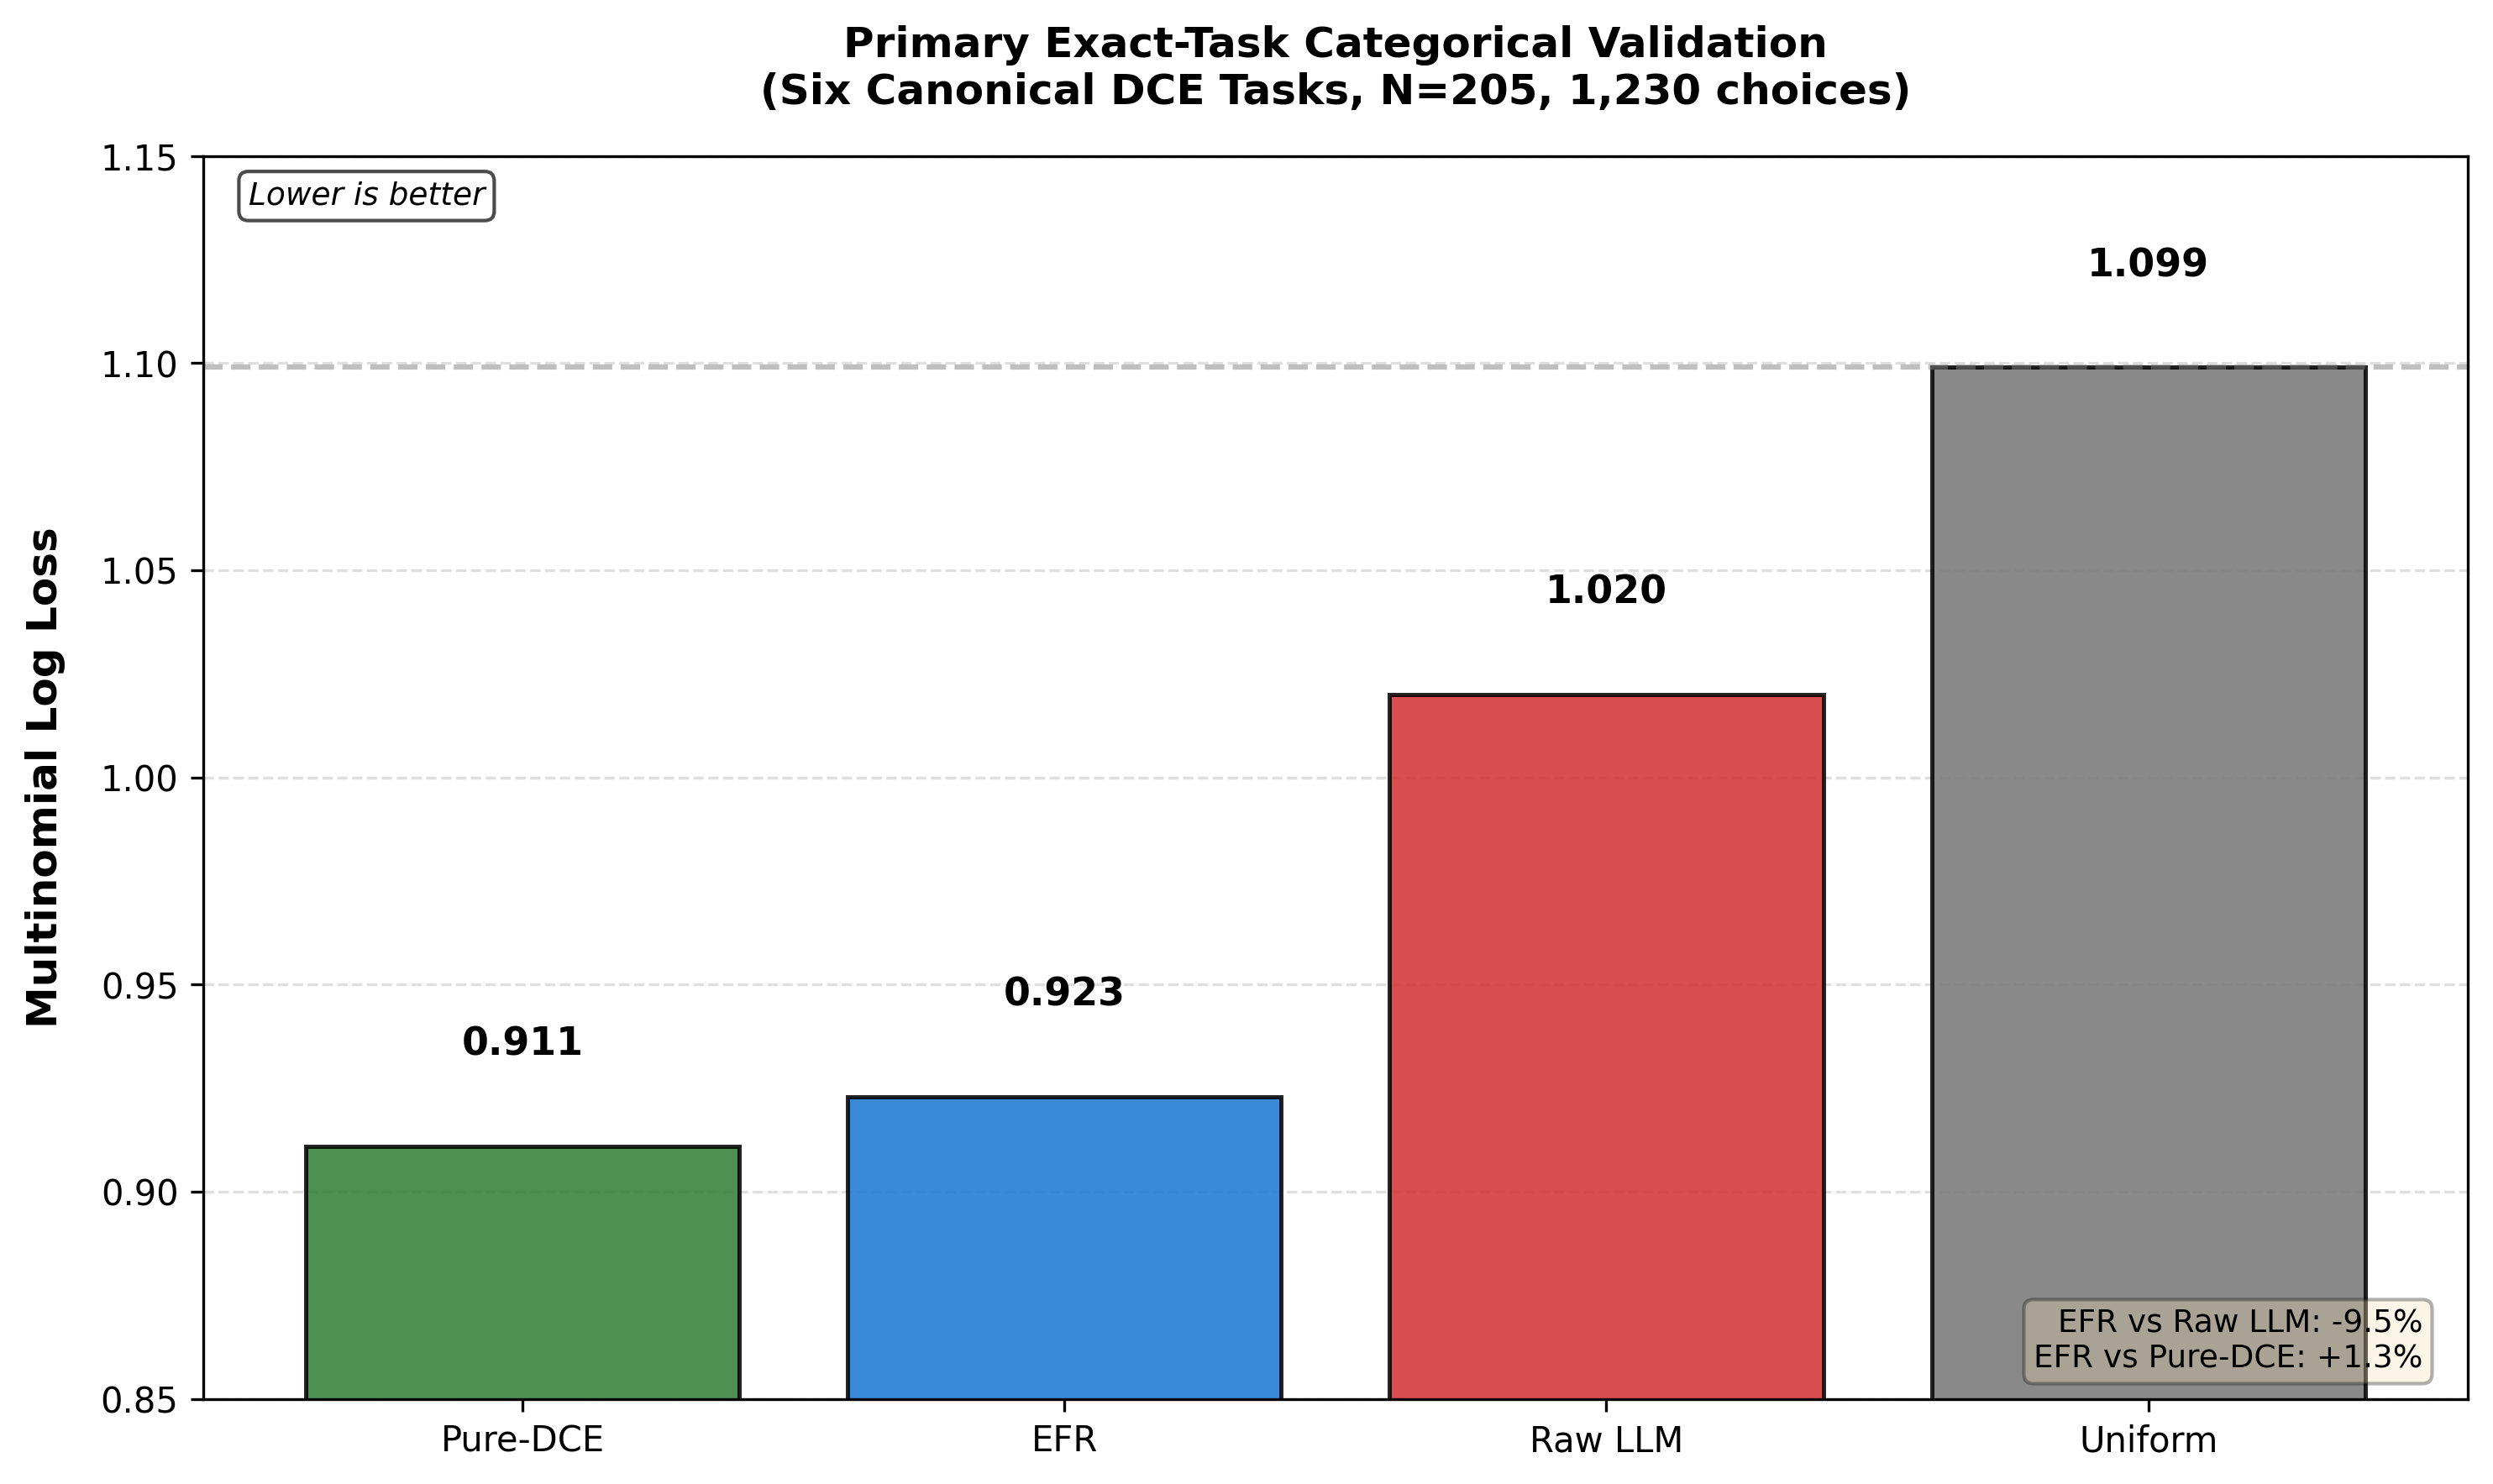
\includegraphics[width=0.98\textwidth]{figures/figure_1_heldout_predictive.png}
\caption{Multinomial log loss on held-out DCE tasks ($N=205$). EFR improved versus Raw LLM ($-0.097$; 95\% CI $-0.147$ to $-0.047$); difference from Pure-DCE was small ($+0.012$; 95\% CI $-0.023$ to $+0.047$).}
\label{fig:heldout_predictive}
\end{figure}

\subsection{Implementation and Policy Recommendations}\nopagebreak\label{sec:policy_impl}

\textbf{Significance.} EFR applies an DCE frontier to narrative-policy evaluation. The $\lambda=0.25$ anchor bounds LLM deviation. OOD evaluation shows structural consistency (monotonicity, rank order), but this is a constraint effect, not evidence of LLM accuracy for novel scenarios. EFR is a narrative-extension wrapper, not a DCE replacement or LLM validation. Implementation requires no model retraining: an analyst estimates a 6-parameter grouped/conditional logit from an DCE, generates LLM predictions, and blends them through $\pi_{\mathrm{adj}} = \lambda \pi_{\mathrm{LLM}} + (1-\lambda) P_{\mathrm{emp}}$ ($\lambda = 0.25$). Three policy implications follow. \emph{With a DCE}, EFR provides a path from evidence to narrative policy simulation. \emph{Without a DCE}, the framework is not a substitute for stated-preference data. \emph{Best for early-stage screening}, not high-stakes final decisions. The permutation analysis indicates that incremental DCE-aligned rank structure in LLM component is model-dependent: it was detectable for DeepSeek V4 Pro and MiroThinker, but not for Qwen2.5-72B.



\subsection{Conclusion}\nopagebreak\label{sec:conclusion}

EFR anchors LLM outputs to DCE estimates without retraining. Held-out validation ($N=205$): EFR improved log loss versus Raw LLM and approached Pure-DCE (1.3\%). On the 64-state grid, EFR reduced waiting-time violations (Table~1). OOD evaluation shows structural consistency (Supp. Mat.). EFR is a constrained narrative-extension wrapper; the empirical reference supplies the signal. Whether narrative extension improves behavioral accuracy on novel scenarios awaits human ground truth. Four directions are planned future work: (i) replication across additional diseases, jurisdictions, and policy domains; (ii) exploration of non-convex anchoring mechanisms (e.g., mixture-of-experts gating); (iii) quasi-experimental validation with human ground truth on out-of-design narrative scenarios; and (iv) dynamic DCE updating, in which the empirical frontier is re-estimated and the blending weight re-calibrated as new stated-preference data accumulate.

\clearpage
\section*{References}
\addcontentsline{toc}{section}{References}

\renewcommand{\refname}{}
\bibliographystyle{unsrtnat}
\bibliography{references_round3}



\clearpage
\section*{Supplementary Materials}
\addcontentsline{toc}{section}{Supplementary Materials}

The following supplementary materials accompany this manuscript and are available in the online appendix.

\textbf{A. Tables}
\begin{itemize}\setlength{\itemsep}{0pt}
\item \textbf{Table S1.} Observed EFR Spearman $\rho$ versus uniform-noise and permutation nulls on the 64-state grid.
\item \textbf{Table S2.} LLM decoding and endpoint parameters used in the main, supplementary, and stress-test evaluations.
\item \textbf{Table S3.} \emph{Administered} DCE attribute levels: waiting time $\{0, 1, 3, 6\}$ months (4 real design levels; the raw coded data contain a single 1-row outlier at wait $= 2$ months from Respondent 1 only, which was excluded from all analyses before sample-size calculations). The analytic sample contains 18,485 alt-rows (6,162 choice tasks $\times$ 3 alternatives minus 1 anomalous row). All 1,027 respondents completed the same six choice tasks; task presentation order was randomized across respondents to mitigate order effects. Each task presented two non-opt-out alternatives and an opt-out alternative. The held-out validation subsample ($N=205$ respondents) contains 1,230 valid tasks (205 $\times$ 6; the anomalous row was from Respondent 1, who was not in the held-out subsample). The design contained six unique administered choice tasks and 12 non-opt-out profiles per respondent (12 unique non-opt-out profiles in the design; $12{,}324 = 1{,}027 \times 12$ profile instances across all respondents). The 12 administered non-opt-out attribute combinations per respondent enumerate 12 of the $3 \times 3 \times 3 \times 2 \times 4 = 216$ non-opt-out candidate cells (5.6\% per-respondent coverage).
\item \textbf{Table S4.} Attribute coding dictionary: DCE questionnaire display, estimation coding, 64-state evaluation-grid coding, and coefficient unit definitions.
\item \textbf{Table S5.} Conditional-logit estimates (corrected 6-parameter specification) used to construct the empirical choice frontier. Standard errors from BFGS Hessian; bootstrap 95\% confidence intervals for the 6 coefficients.
\item \textbf{Table S6.} $\lambda$-sensitivity for frontier-alignment diagnostics on the 64-state grid. Pure-DCE baseline, unconstrained LLM, and EFR Anchor evaluated across $\lambda \in \{0.00, 0.10, 0.20, 0.25, 0.30, 0.40, 0.50, 0.60, 0.70, 0.80, 0.90, 1.00\}$.
\item \textbf{Table S7.} $\lambda$-sensitivity for partial-support grid-overlap diagnostic on the 813 \emph{alternative-level} rows subset (from 205 held-out respondents). Matching is on three focal attributes (waiting time, efficacy, side-effect burden) only; cash incentive and vaccine origin are not matched between the DCE alternatives and the LLM grid. Alt-level binary log loss, Brier score, and AUC across $\lambda$.
\item \textbf{Table S8.} Data-scaling ablation: EFR Anchor ($\lambda=0.25$) vs.\ unconstrained LLM across training fractions ($30\%, 50\%, 70\%, 100\%$).
\item \textbf{Table S9.} Parse success rates across models and experiment scales.
\item \textbf{Table S10.} Runtime summary for full-scale unconstrained LLM generation.
\item \textbf{Table S11.} Policy Ranking Consistency (PRC) relative to the Pure-DCE reference; descriptive structural diagnostic, no significance test.
\item \textbf{Table S12.} Respondent-level paired cluster bootstrap for exact-task multinomial log loss (six canonical tasks; $N = 205$ respondents).
\item \textbf{Table S13.} Bootstrap intervals for selected frontier-alignment diagnostics.
\item \textbf{Table S14.} Attribute-level mapping between the administered DCE design and the 64-state LLM evaluation grid. The matched subset is restricted to cells where the DCE design level and the grid level coincide as a \texttt{float} value (no rescaling, no interpolation).
\item \textbf{Table S15.} Covariate balance between matched and unmatched held-out subsets.
\item \textbf{Table S16.} Primary exact-task multinomial held-out log loss on six canonical DCE tasks ($N = 205$ respondents, 1,230 choices). Pure-DCE, EFR, Raw LLM, and uniform baseline.
\end{itemize}

\textbf{B. Figures}
\begin{itemize}\setlength{\itemsep}{0pt}
\item \textbf{Figure S1.} Data-scaling ablation: EFR Anchor ($\lambda = 0.25$) evaluated across DCE training shares ($30\%, 50\%, 70\%, 100\%$); companion to the data-scaling narrative in Appendix~G.
\end{itemize}

\textbf{C. Replication Materials}

Replication materials are available at \url{https://github.com/REDACTED/behavioral-digital-twins}, including: the questionnaire, code, de-identified aggregate/grid-level inputs, model outputs, and derived analysis datasets required to reproduce the reported LLM and frontier-alignment analyses. Individual-level DCE responses are not publicly released because of participant confidentiality.

\appendix
\end{document}